% C.21 □ABCD, AC=12, BD=16, AB=10, O 交点
\documentclass[tikz,border=4pt]{standalone}
\usepackage{ctex}
\usepackage{amsmath}
\usetikzlibrary{calc, arrows.meta}
\begin{document}
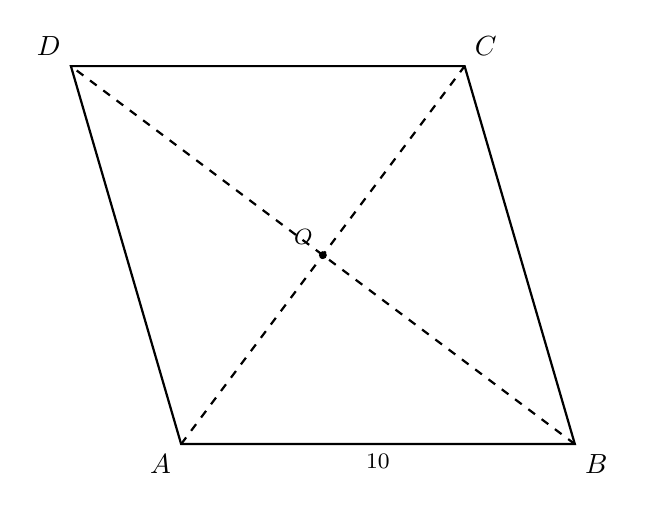
\begin{tikzpicture}[scale=0.5, thick]
  \coordinate (A) at (0,0);
  \coordinate (B) at (10,0);
  % we need a parallelogram with diagonals 12 and 16. By identity: AC^2+BD^2=2(AB^2+AD^2) → 144+256=2(100+AD^2) → AD^2=100 → AD=10! So actually rhombus-like.
  % Place D such that AD=10 and diagonal BD=16. D=(dx,dy), dx^2+dy^2=100, (dx-10)^2+dy^2=256 → -20 dx+100=156 → dx=-2.8, dy=sqrt(100-7.84)=sqrt(92.16)=9.6
  \coordinate (D) at (-2.8, 9.6);
  \coordinate (C) at (7.2, 9.6);
  \coordinate (O) at ($(A)!0.5!(C)$);
  \draw (A) -- (B) -- (C) -- (D) -- cycle;
  \draw[dashed] (A) -- (C);
  \draw[dashed] (B) -- (D);
  \filldraw (O) circle (2pt);
  \node[below left] at (A) {$A$};
  \node[below right] at (B) {$B$};
  \node[above right] at (C) {$C$};
  \node[above left] at (D) {$D$};
  \node[above left, font=\footnotesize] at (O) {$O$};
  \node[font=\footnotesize, below] at (5,0) {$10$};
\end{tikzpicture}
\end{document}
